%Sample Lab report format, ECE112

\documentclass[11pt, oneside]{article}
\usepackage{graphicx}
\usepackage{epstopdf}  %this is new
\usepackage{titling}  %allows altering the title spacing
\usepackage{mathtools}
\usepackage{amsmath} %better math capability
\usepackage{gensymb} %for misc symbols like degrees kelvin
\usepackage{xfrac}   %for inline fractions within text
\usepackage{caption}
\usepackage{subcaption}
\usepackage{float}   %lets you have non-floating floats
\floatstyle{plain}
\restylefloat{figure}
\usepackage{fullpage}%smaller margins
\usepackage{framed,color} %for text frames in color
\definecolor{shadecolor}{rgb}{0.9,0.9,0.9} % for code text frames in grey
\usepackage{url} %for typesetting urls
\renewcommand*\rmdefault{ppl}   %use pallatino font
\usepackage{multicol} %for multi column layout, added by caoji 1/8/14
%\usepackage{vwcol}
\usepackage{multirow}
\usepackage{dcolumn} %Aligning columns at decimal points using dcolumn
\newcommand{\uline}[1]{\rule[0pt]{#1}{0.4pt}}% Fill this blank
\usepackage{listings} %allow includes of source code files

%\lstset{basicstyle=\scriptsize,keepspaces=true,frame=single,backgroundcolor=\color{shadecolor}}
\lstset{basicstyle=\ttfamily\scriptsize,breaklines=true}
\lstset{framextopmargin=50pt,backgroundcolor=\color{shadecolor}}

\title{\vspace{-3.0cm}ECE112 Lab Report - Linux and Spice Simulation lab}
\author{Abhi Balijepalli}

%\date                     %comment this out if you want the date printed.
\setlength\parindent{0pt}  %no indents on any paragraphs
\setlength\fboxsep{8pt}    %bigger separaration for figure boxes

\begin{document}
\maketitle

\section*{Lab 6a - ECE112}

\subsection*{Here is what I did}
 
This lab was about running the spice simulator and printing some results
with latex. My results from this lab are shown in figure \ref{fig:simplot}.

\begin{figure}[H]
%trim setting order: left, bottom, right, top
\center
\fbox{{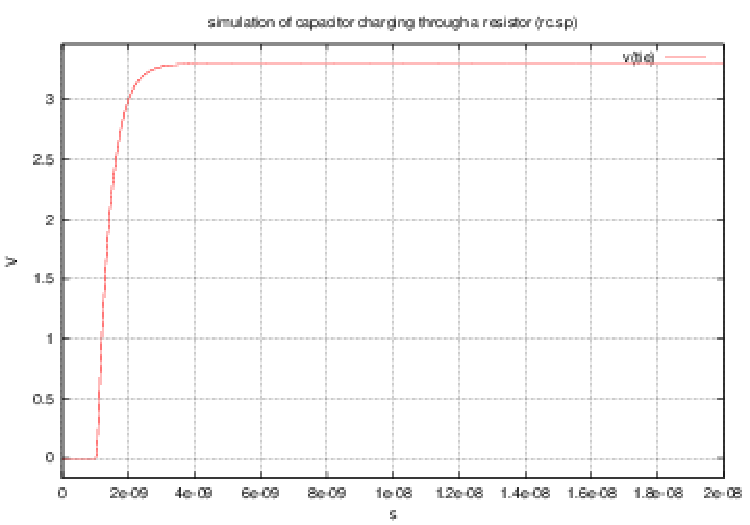
\includegraphics[scale=0.7, trim = 0mm  0mm  0mm  0mm, clip=true]{sim_output.pdf}}}
\caption{\label{fig:simplot}RC Simulation}
\end{figure}

\subsection*{Spice netlist}

Here is the spice input file I used:
\vspace{3mm}
\lstinputlisting{rc.sp}

\vspace{3mm}
Signed: \hspace{1mm}
%\vspace{0.1in} \\
\uline{1.5in} \vspace{0.2in} \\

\end{document}
